\documentclass[10pt,letterpaper,addpoints]{exam}
\usepackage[utf8]{inputenc}
\usepackage[spanish,es-noshorthands]{babel}
\usepackage{hyperref}
\usepackage{amsmath}
\usepackage{amsfonts}
\usepackage{amssymb}
\usepackage{graphicx}
\usepackage{tikz}
\usepackage{multicol}
\usepackage[width=7in,height=9.5in]{geometry}
%\printanswers
\begin{document}
\title{\begin{minipage}{.2\textwidth}
        
\includegraphics[height=1.75cm]{Images/logo-colegio.png}
       \end{minipage}
\begin{minipage}{.55\textwidth}
 \begin{center}
Prueba bimestral ii\\Matemáticas $6^{\circ}$
\end{center}
\end{minipage}
\begin{minipage}{.2\textwidth}

\includegraphics[height=1.75cm]{Images/logo-sed.png} 
\end{minipage}
}
\author{Germ\'{a}n Avendaño Ram\'{i}rez\\Lic. Matemáticas U.D., M.Sc. U.N.}
\date{}
\maketitle
\begin{center}
\fbox{\fbox{\parbox{5.5in}{\centering
Instrucciones}}}
\end{center}
\vspace{0.1in}
\makebox[\textwidth]{Nombres: \hrulefill, curso:\underline{\hspace{48pt}}, fecha:\underline{\hspace{3cm}}}
\begin{multicols}{2}
\begin{questions}
\uplevel{Los relojes muestran las horas de iniciación y terminación del recreo en un colegio.}
\begin{center}
 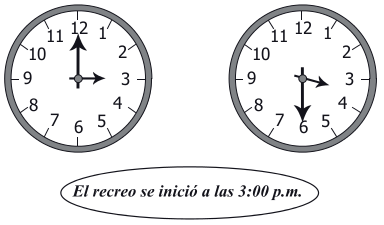
\includegraphics[scale=.8]{Images/relojes.png}
 \end{center} 
\question El recreo finalizó a las 3:30 p.m. ¿Cuánto avanzó el minutero desde que se inició el recreo?
\begin{choices}
\choice Un cuarto de vuelta.
\CorrectChoice Media vuelta.
\choice Tres cuartos de vuelta.
\choice Una 30 vuelta.
\end{choices}
%Pregunta
%\begin{oneparchoices}
%\choice[1] Nunca
%\end{oneparchoices}
%\answerline
%\end{questions}
%cuadro de puntajes
%\begin{center}
%\gradetable[h][pages]
%\end{center}
\end{multicols}
\end{document}